\usepackage{biblatex}\chapter{Methodology}\label{ch:methodology}

This chapter outlines the methodological approach taken to bridge the identified gaps between values-driven impact measurement and practical, scalable tools supported by artificial intelligence.
Grounded in the context of the Public Value Hub in Leipzig, this research combines qualitative inquiry with experimental AI applications to explore how language models can support meaning-making in public innovation.

\section{Research Design}\label{sec:research-design}

The study follows a mixed-methods, exploratory design, combining:

\begin{itemize}
    \item Qualitative research, including semi-structured stakeholder interviews and participatory workshops, to identify core needs and values in public sector impact work.
    \item Experimental development of AI-supported tools, specifically using large language models (LLMs) for natural language understanding and semantic analysis.
\end{itemize}

The overall approach is informed by design science and action research traditions, aimed at producing both understanding and actionable prototypes in a real-world innovation setting.

\section{Qualitative Inquiry}\label{sec:qualitative-inquiry}

Interviews were conducted with public sector innovators and researchers affiliated with the Public Value Hub and the Public Value Academy.
These engagements explored:

\begin{itemize}
    \item Current impact measurement challenges in innovation projects,
    \item How concepts like \textbf{public value} are interpreted in practice,
    \item Stakeholder needs for sense-making, learning, and transparency in evaluation.
\end{itemize}

Thematic analysis of transcripts was used to extract design criteria for the AI components — particularly around interpretability, flexibility, and the need to reflect both quantitative and narrative dimensions of impact.

\section{LLM-Based Tool Development}\label{sec:llm-based-tool-development}

This section describes the development of AI-supported tools designed to augment — not automate — value-driven decision-making in public innovation.

\subsection{Narrative Analysis of Pitch Decks}\label{subsec:narrative-analysis-of-pitch-decks}

To support early-stage project evaluation, pitch decks from public innovation teams were analyzed using an LLM (e.g., OpenAI’s GPT-4).
The model was prompted to extract:

\begin{itemize}
    \item Key impact themes,
    \item Evidence of alignment with public value dimensions,
    \item Indicators of potential long-term benefit or stakeholder inclusion.
\end{itemize}

Outputs were compared across cases to test for consistency and relevance, serving as a prototype for narrative-based impact reviews.

\subsection{Semantic Similarity Search Across Frameworks}\label{subsec:semantic-similarity-search-across-frameworks}

A corpus of over \todo{check how many frameworks we tend to implement}40~\todo{add list of frameworks to annex} different evaluation frameworks, sourced from academia, government, and practice, was compiled and pre-processed.
The goal was to support innovation teams in selecting or aligning with existing approaches.

Using sentence embeddings (via BERT or Sentence-Transformers), a similarity search tool was built to allow users to query their own impact statements or goals against this corpus to discover:

\begin{itemize}
    \item Conceptual overlaps,
    \item Implicit values in each framework,
    \item Alternative metrics or lenses for evaluation.
\end{itemize}

This addressed a recurring concern in interviews: that existing frameworks are often applied blindly or bureaucratically, without being interrogated for fit or value alignment.

\subsection{Clustering and Thematic Grouping of Narratives}\label{subsec:clustering-and-thematic-grouping-of-narratives}

To identify recurring themes in unstructured narratives emerging from public innovation contexts — such as project proposals, workshop transcripts, or citizen inputs — a semantic clustering pipeline was implemented.
The goal was to surface latent topics reflecting common challenges, priorities, or value framings across diverse projects.

\textbf{Embedding Generation:} Narrative inputs were converted into dense vector representations using OpenAI’s \texttt{text-embedding-ada-002} model~\parencite{OpenAI2023Embedding}, selected for its ability to capture rich semantic relationships beyond surface lexical similarity~\parencite{Reimers2019SentenceBERT}.

\textbf{Dimensionality Reduction:} To reduce noise and improve interpretability, embeddings were optionally projected into a lower-dimensional space using Uniform Manifold Approximation and Projection (UMAP)~\parencite{McInnes2018UMAP}, which preserves local and global data structure better than PCA~\parencite{vanDerMaaten2008tSNE}.

\textbf{Clustering:} Hierarchical Density-Based Spatial Clustering of Applications with Noise (HDBSCAN)~\parencite{Campello2013HDBSCAN} was employed, which suits variable-density clusters and noisy data typical in qualitative text corpora.

\textbf{Cluster Interpretation:} Representative documents from each cluster were summarized using GPT-4~\parencite{OpenAI2023GPT4} to generate interpretable labels, leveraging advances in large language models for thematic summarization~\parencite{Bamman2020LLMTextMining}.

\textbf{Use in Downstream Tasks:} Thematic clusters informed subsequent pipeline stages such as KPI generation, and facilitated stakeholder reporting by providing structured overviews of diverse narrative inputs, enhancing transparency and reflection~\citep{Braun2019ThematicAnalysis,Feng2019MixedMethodsNLP}.


\begin{figure}[H]
    \centering
    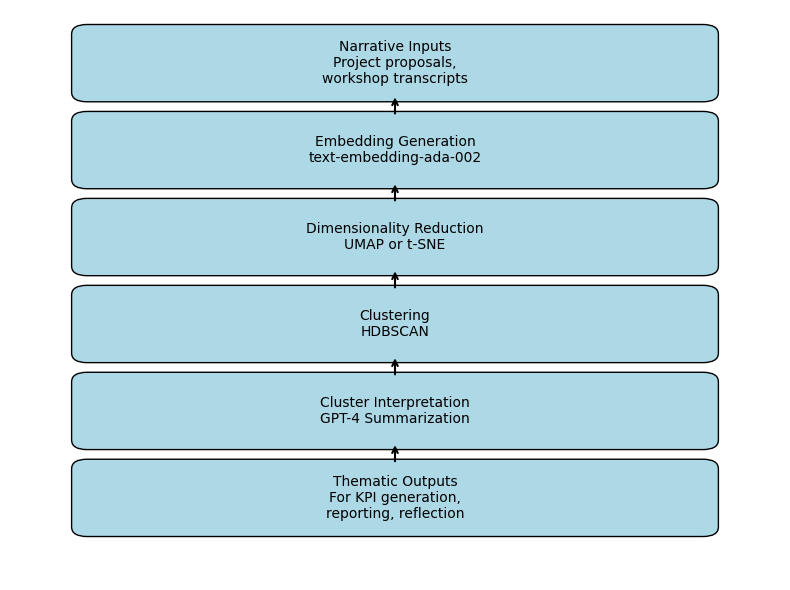
\includegraphics[width=0.9\textwidth]{../fig/clustering_pipeline}
    \caption{Semantic Clustering Pipeline for Narrative Inputs}
    \label{fig:clustering-pipeline}
\end{figure}

% Continue with text referencing Figure~\ref{fig:clustering-pipeline}

\subsection{Automated KPI Derivation via LangGraph Pipelines}\label{subsec:kpi-pipeline}

To explore how generative AI can support structured evaluation in public innovation, a modular pipeline was developed using the LangGraph framework — a tool for orchestrating large language models in stateful workflows.
The objective was to generate context-sensitive, auditable Key Performance Indicators (KPIs) based on unstructured pitch materials, reflecting relevant dimensions of public value and providing measurable evaluation anchors.

The pipeline integrates multiple AI-supported stages:

\begin{enumerate}
    \item \textbf{Input Parsing and Structuring:} Raw pitch decks (PDFs) are processed using AI-based document parsing. \\Structured outputs are extracted using \texttt{LangChain}’s schema-based tools and validated via Pydantic models~\parencite{LCStructuredOutputs2025}.

    \item \textbf{Problem Statement Generation:} A language model generates a concise problem statement and a summary profile based on extracted content.\\ This can also be manually edited or entered directly by the user.

    \item \textbf{Metric and Leverage Point Extraction:} For each defined problem, AI identifies one or more relevant metrics and potential leverage points, guided by both domain knowledge and similarity search against curated sources.

    \item \textbf{Extended Contextual Fields:} Additional structured fields enrich the problem context, including:
    \begin{itemize}
        \item Beneficiaries and their needs
        \item Target customer groups
        \item Systemic framing of the problem
        \item Competitive landscape
    \end{itemize}

    \item \textbf{Solution Mapping:} AI summarizes the proposed solution using multiple structured prompts, including:
    \begin{itemize}
        \item Solution summary and visual description
        \item USP and strengths
        \item Impact business model
        \item Claims, solution tree(s), and logic of change
    \end{itemize}

    \item \textbf{Impact Framing:} The pipeline captures desired outcomes and long-term impacts using the IOOI model (Inputs, Outputs, Outcomes, Impact), supporting both existing impact data and forward-looking impact goals~\parencite{IOOIFrameworkRef2023}.

    \item \textbf{SDG Alignment:} The structured problem and solution descriptions are semantically mapped to relevant Sustainable Development Goals (SDGs) using a GPT-4 classifier~\parencite{UNSDG2024}.

    \item \textbf{Indicator Retrieval and Critique:} A vector similarity search (via pgvector) identifies candidate indicators from a curated indicator database~\parencite{LCSimilaritySearch2025}.
    \item These are passed through a critique model to assess fit and refine relevance.

    \item \textbf{KPI Generation:} KPIs are proposed for each problem-solution pair, incorporating name, measurement logic, targets, and context sensitivity. Each KPI is evaluated using a rubric assessing clarity, measurability, and alignment.

    \item \textbf{Audit and Regeneration:} If the KPI quality score falls below a set threshold (e.g., $>$80\%), the generation cycle is repeated~\parencite{LCGraphBuilding2025}.

    \item \textbf{Transparency Trace:} The full decision path and rationale for KPI generation are captured using explainable AI tooling (e.g., SHAP)~\parencite{ShapXAI22025}, enabling transparency in impact evaluation.
\end{enumerate}

The pipeline was tested using anonymized or synthetic pitch materials from early-stage social innovation projects.
The modular design enables flexible adaptation across sectors, while maintaining a transparent and reflexive architecture appropriate for value-driven impact work.

\begin{figure}[H]
    \centering
    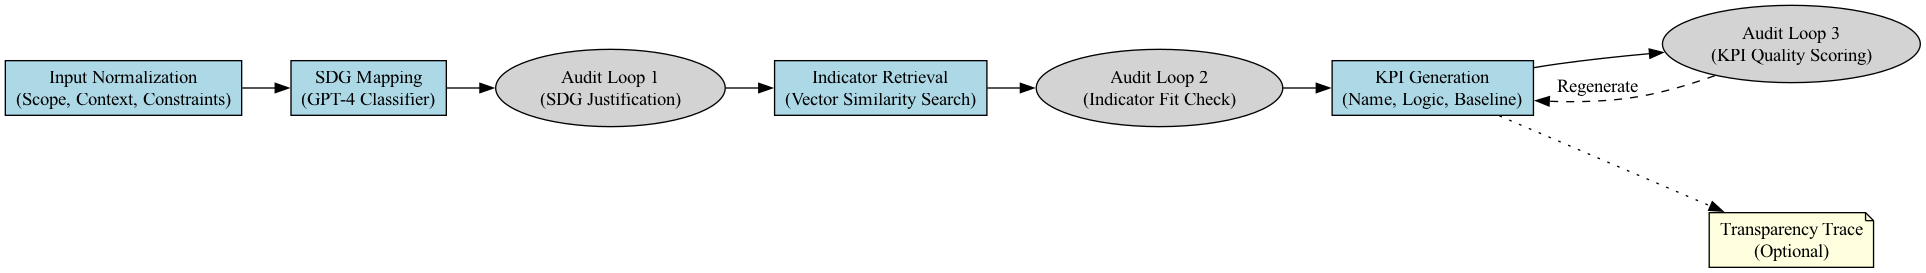
\includegraphics[height = 0.9\textheight]{../fig/langgraph_pipeline}
    \caption{LangGraph pipeline for automated KPI derivation and impact structuring}
    \label{fig:langgraph-pipeline}
\end{figure}

\section{Integration into Public Value Academy Platform}\label{sec:integration-into-public-value-academy-platform}

To test applicability, these AI tools were designed for compatibility with the existing Public Value Academy digital infrastructure.
This platform supports workshops and guided reflection around public value and innovation — making it a suitable space to prototype and iteratively improve language-based evaluative tools.

\section{Evaluation Strategy}\label{sec:evaluation-strategy}

Given the exploratory nature of this work, a formative evaluation approach was adopted.
Tools were tested using anonymized project documents, workshop materials, and synthetic inputs.
Early feedback was gathered through user walkthroughs and informal interviews with practitioners and researchers.

Evaluation criteria included:

\begin{itemize}
    \item Usefulness and clarity of AI-generated insights,
    \item Perceived alignment with stakeholder values and expectations,
    \item Potential for embedding in existing impact workflows without undermining deliberation.
\end{itemize}

\section{Ethical Considerations}\label{sec:ethical-considerations}

All qualitative research participants provided informed consent, and data was handled in accordance with GDPR and institutional ethical guidelines.

To ensure responsible use of AI, all computational components were designed to support transparency, interpretability, and human oversight.
This was implemented through a combination of justification-based outputs, audit loops, and optional explainability tools.

Justification generation was embedded in key stages of the LangGraph pipeline — particularly during SDG classification, indicator selection, and KPI generation — allowing models to provide rationale for their outputs.
These justifications served both for internal audit loops and as prompts for human-in-the-loop (HITL) intervention, especially during early-stage deployment~\parencite{ribeiro2016should, Holzinger2016HITL}.

This approach draws from Explainable AI (XAI) principles, aiming to make opaque model reasoning more transparent to users and stakeholders~\parencite{dwivedi2023explainable}.
Where appropriate, explainability methods such as SHAP were used to surface feature-level insights and support model interpretation~\parencite{lundberg2017shap}.

These measures align with policy frameworks such as the EU AI Act and OECD AI Principles, which call for trustworthy AI systems that preserve human agency, ensure traceability, and enable contestability of automated decisions~\parencite{euai2023, oecd2022ai}.

In summary, this setup reflects the project's core principle: AI should augment — not replace — human judgment in complex, value-laden public sector contexts.